\subsubsection{Raster Data Services}
\index{Baumann, Peter}
\paragraph{Research Team}
Peter Baumann (Professor), Angelica Garcia Gutierrez (PhD Student)\\

Raster data occur in various dimensions, be they observed phenomena or generated data
sets. Examples comprise satellite imagery and mapping, geo physics and exploration,
medical imagery, engineering data, and statistics data. A key property they have in common
is their extreme volumes, often Giga- to Petabyte per object.

With the advent of sufficiently large disk capacities data providers more and more tend to
publish such large Multidimensional Discrete Data (MDD) - GoogleEarth is a prominent
example. Generally such services are implemented in an ad-hoc manner, and consequently
offer limited functionality (such as GoogleEarth: zoom and pan on satellite
maps). However, flexible, value-added data navigation and analysis requires more, both for
experts (such as exploration engineers) and the general public (where internally complex
functionality like local weather prediction obviously should be wrapped for easy access).

MDD database and Web service support raises new questions on all levels: conceptually,
formal models are needed to describe data and services; query languages resp. request
interfaces need to be designed based on these foundations. Efficient implementation,
including optimizing query evaluation and storage structures, is needed. The high volume
suggests to include tape robots as nearline storage facilities. Last but not least
services for as many application domains as possible need to be realized to gain domain
understanding and to evaluate service implementations.

In our research we investigate on the principles of MDD management based on the rasdaman
("raster data manager") system acting as a research platform. Application domains
inspected are mainly stemming from earth system research, such as 2-D to 4-D remote
sensing, exploration, marine, and climate data. As a byproduct we are actively engaged in
the Open GeoSpatial Consortium where we contribute to the standardization of geo raster
services.

\paragraph{Highlights}

An important work package is contribution to geo raster service
standardization in the Open GeoSpatial Consortium (OGC,
\url{http://www.opengis.org}). We are actively contributing in the
Web Coverage Service (WCS) Revision Working Group where the
substantially revised WCS version 1.1 has been finished by the end
of 2006. Based on the experience gained there and the WCS
shortcomings spotted we have propose the concept of a Web Coverage
Processing Service (WCPS); Figure~\ref{fig:ndvi} exemplifies usage
of WCPS by dynamically deriving the NDVI of a Landsat satellite
scene; the NDVI I of an image is defined as I=(nir-red)/(nir+red),
in the right image it is thresholded as $I>0.6$. In June 2006, WCPS
has been lifted to a Best Practice Paper (which implies OGC
endorsement), it is estimated that WCPS can become a Draft Standard
end of 2006 / beginning of 2007, and a full standard by summer 2007.
Several institutions, among them German mapping (AdV) and
geophysical institutions (such as BGR) have expressed their
interest.

In parallel to the conceptual work on WCS and WCPS, our group implements both
services. Prototypes have been demonstrated at various occasions in 2006, among them OGC
Technical Commitee meetings. For 2007 it is planned to set up large-scale services fo
thorough evaluation prior to freezing the final standard document.

The GALEON (Geo-interface to Atmosphere, Land, Earth, Ocean, NetCDF) project launched in
2005 meantime has become an OGCnetwork (\url{http://www.ogcnetwork.net/galeon}); besides
contributing to WCS requirements it is starting now to hands-on evaluate the new WCS
1.1. IUB will contribute our WCS implementation, which is under work,

As part of the IRCCM project (\url{http://www.irccm.org}) and in collaboration with IUB's geo group and
AWI Bremerhaven, a standards-based open service for marine research data has been set up
which combines bathymetry data and video mosaics acquired by a French underwater
robot. Data describe an underwater volcano in the Norwegian Atlantic area known as
Hakon-Mosby. This service is the first step towards a more comprehensive multi-sensor
fusion service between IUB and AWI.

For the ICSU CODATA (Committee on Data in Science and Technology) a German section has
been established as an "e.V." and has been accredited with CODATA International. As a side
effect of this work, several fruitful research contacts have emerged, such as with the
Chinese Academy of Science (see above).

\begin{figure}[ht]
  \begin{center}
     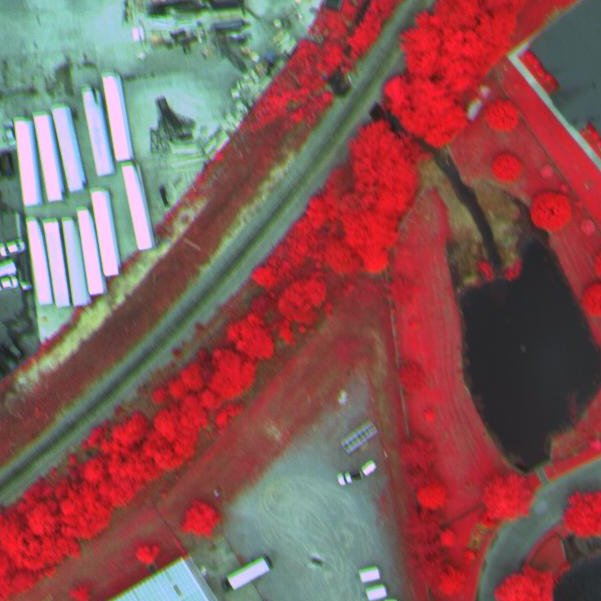
\includegraphics[width=3.5cm]{ndvi-1.jpg}
     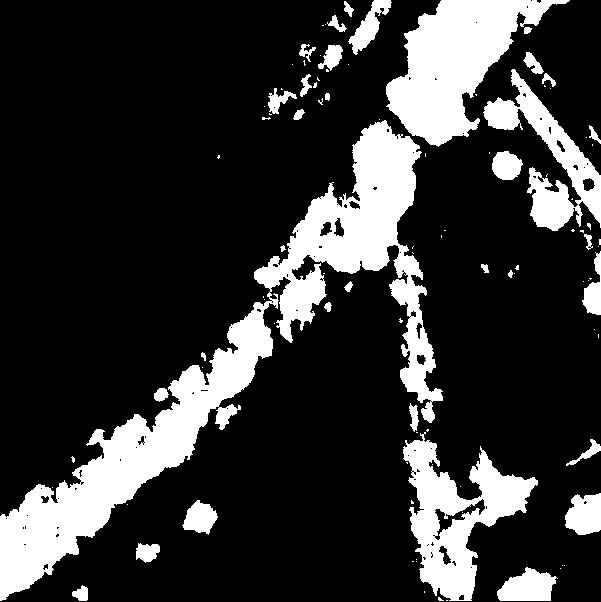
\includegraphics[width=3.5cm]{ndvi-2.jpg}
    \caption{The Normalized Difference Vegetation Index (NDVI) as a database / Web
      service query (rasdaman screen shots).}\label{fig:ndvi}
   \end{center}
\end{figure}

\paragraph{Collaborations}

In 2006 several new international research cooperations have been established:
\begin{enumerate}
\item {\sl Universidade de Campinas (Unicamp), Campinas, Brazil}

  Prof. Claudia Bauzer Medeiros is Head of the Laboratory of Information Systems (LIS) at
  the Institute of Computing, UniCamp, and President of the Brazilian Computer
  Society. With her group she works on advanced Web-based geo services with emphasis on
  agrocultural and environmental applications; to this end there is a long-standing
  relation with the Brazilian Ministry of Agriculture.

  In the collaboration, for which a joint research proposal has been submitted to
  DAAD/Germany and INPe/Brazil, both partners plan to extend Unicamp's geo services with
  IUB's raster services, based on the open OGC standards. The resulting system will be
  exercised in real life operation. Evaluation results will be brought into OGC to give
  feedback to the standards developers.

\item {\sl Universidad de Sinaloa, Sinaloa, Mexico}

  Dr. Ines Fernando Lopez Vega, who in 2004 has received his PhD from University of
  Arizona at Tucson, is building up his research on image time series
  evaluation. Collaboration is foreseen combining his interests with our raster service
  research and Michael Kohlhase's work on Semantic Web services.

  Collaboration was initiated in Fall 2006 with a visit of Dr Lopez Vega in the course of
  his co-supervision of Angelica Garcia Gutierrez's PhD work.

\item {\sl Chinese Academy of Sciences and Jilin University, Changchun, China}

  Prof. Liu Chuang plays an important role in China when it comes to provision and
  exploration of remote sensing data. Among others, she is Vice Director of the Institute
  of Geography and Natural Resources (IGNR) and director of the Spatial Data Commission,
  the Chinese Association of Geographic Information System (CAGIS), and Secretary General
  of a Working Group of Remote Sensing and Data Information Systems (RS/DIS).

  IUB, IGNR und Jilin University plan joint activities in the field of open
  standards-based geo services on high-volume in situ and remote sensing data, based on
  rasdaman. As a real life application IGNR's 100+ TB data archive of Chinese satellite
  imagery collected over several years will serve, today stored in hundreds of DVDs,
  unavailable to the researcher community. The Chinese National Disaster Reduction Center
  will be one of the first users, with application scenarions being river floods and
  earthquakes.
\end{enumerate}


Several tutorials have been given on the topic of raster services:
\begin{enumerate}
\item CODATA 2006 Conference, Beijing (3 hrs)
\item 1st International Symposium on Cooperation and Promotion of Information Resources in
  Science and Technology (under the auspices of the Chinese Ministry of Science and
  Technology), Beijing (2 hrs)
\item 19th IFIP World Computer Congress, Santiago de Chile (3 hrs)
\end{enumerate}

%\paragraph{Publications}

%\begin{description}
\nocite{PB:comogis,PB:codata,PB:fig}
%\end{description}
%%% Local Variables:
%%% mode: latex
%%% TeX-master: "report"
%%% End:
